\normaltrue
\correctiontrue

%\UPSTIidClasse{11} % 11 sup, 12 spé
%\newcommand{\UPSTIidClasse}{11}


\exer{Mouvement TT -- $\star$ \label{C2:07:03}}
\setcounter{question}{0}\UPSTIcompetence[2]{B2-14}
\UPSTIcompetence[2]{B2-15}
\UPSTIcompetence[2]{C2-07}
\index{Compétence B2-14}
\index{Compétence B2-15}
\index{Compétence C2-07}
\index{Torseur des actions mécaniques transmissibles}
\index{Torseur d’une action mécanique extérieure}
\index{Principe fondamental de la statique}
\index{PFS}
\index{Mécanisme à 2 translations}
\ifcorrection
\else
\marginnote{\textbf{Pas de corrigé pour cet exercice.}}
\fi

\ifprof
\else
Soit le mécanisme suivant. On note $\vect{AB}=\lambda(t)\vect{i_0}$ et $\vect{BC}=\mu(t)\vect{j_0}$.
$G_1 = B$ désigne le centre d'inertie de \textbf{1},et $m_1$ sa masse. %et $\inertie{G_1}{1}=\matinertie{A_1}{B_1}{C_1}{0}{0}{0}{\bas{1}}$; 
$G_2 = C$ désigne le centre d'inertie de \textbf{2} et  $m_2$ sa masse. % et $\inertie{G_2}{2}=\matinertie{A_2}{B_2}{C_2}{0}{0}{0}{\bas{2}}$.

 Un vérin électrique positionné entre \textbf{0} et \textbf{1} permet de maintenir \textbf{1} en équilibre.
 Un vérin électrique positionné entre \textbf{1} et \textbf{2} permet de maintenir \textbf{2} en équilibre.
 
 On cherche à résoudre le problème \textbf{en statique}.
L'accélération de la pesanteur est donnée par $\vect{g}=-g\vect{j_0}$.



\begin{center}
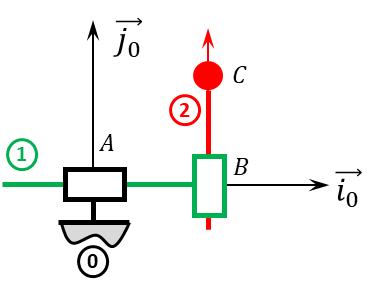
\includegraphics[width=.6\linewidth]{03_TT_01}
\end{center}
\fi

\question{Réaliser le graphe d'analyse en faisant apparaître l'ensemble des actions mécaniques.}
\ifprof
\begin{center}
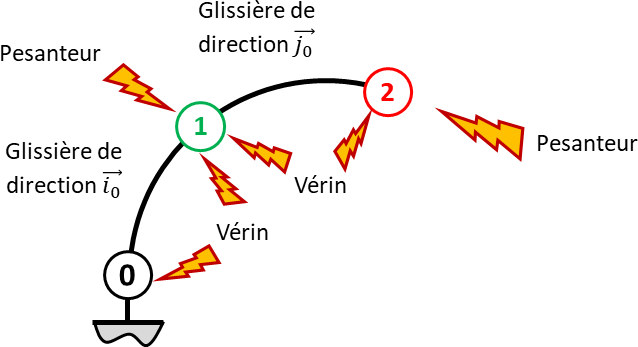
\includegraphics[width=.6\linewidth]{03_TT_01_cor}
\end{center}

\else
\fi




\question{Déterminer l'action à fournir par chacun des vérins pour maintenir le mécanisme à l'équilibre.}
\ifprof
\else
\fi

\question{Déterminer toutes les inconnues de liaison.}
\ifprof
\else
\fi

\ifprof
\question{Donner le torseur de chacune des actions mécaniques.}
\ifprof
\begin{itemize}
\item Glissière entre 0 et 1 : $\torseurstat{T}{0}{1}=\torseurl{Y_{01}\vj{0}+Z_{01}\vk{0}}{L_{01}\vi{0}+M_{01}\vj{0}+N_{01}\vk{0}}{A,\rep{0}}$.
\item Glissière entre 1 et 2 : $\torseurstat{T}{1}{2}=\torseurl{X_{12}\vi{0}+Z_{12}\vk{0}}{L_{12}\vi{0}+M_{12}\vj{0}+N_{12}\vk{0}}{B,\rep{0}}$.
\item Pesanteur sur 1: $\torseurstat{T}{\text{pes}}{1}=\torseurl{-m_1g\vj{0}}{\vect{0}}{B,\rep{0}}$.
\item Pesanteur sur 2: $\torseurstat{T}{\text{pes}}{2}=\torseurl{-m_2g\vj{0}}{\vect{0}}{C,\rep{0}}$.
\item Vérin entre 0 et 1 : $\torseurstat{T}{0_{v1}}{1}=\torseurl{F_1\vi{0}}{\vect{0}}{B,\rep{0}}$.
\item Vérin entre 1 et 2 : $\torseurstat{T}{1_{v2}}{2}=\torseurl{F_2\vj{0}}{\vect{0}}{B,\rep{0}}$.
\end{itemize}
\else
\fi


\question{Simplifier les torseurs dans l'hypothèse des problèmes plans.}
\ifprof
\begin{itemize}
\item Glissière entre 0 et 1 : $\torseurstat{T}{0}{1}=\torseurl{Y_{01}\vj{0}}{N_{01}\vk{0}}{A,\rep{0}}$.
\item Glissière entre 1 et 2 : $\torseurstat{T}{1}{2}=\torseurl{X_{12}\vi{0}}{N_{12}\vk{0}}{B,\rep{0}}$.
\item Pesanteur sur 1: $\torseurstat{T}{\text{pes}}{1}=\torseurl{-m_1g\vj{0}}{\vect{0}}{B,\rep{0}}$.
\item Pesanteur sur 2: $\torseurstat{T}{\text{pes}}{2}=\torseurl{-m_2g\vj{0}}{\vect{0}}{C,\rep{0}}$.
\item Vérin entre 0 et 1 : $\torseurstat{T}{0_{v1}}{1}=\torseurl{F_1\vi{0}}{\vect{0}}{B,\rep{0}}$.
\item Vérin entre 1 et 2 : $\torseurstat{T}{1_{v2}}{2}=\torseurl{F_2\vj{0}}{\vect{0}}{B,\rep{0}}$.
\end{itemize}\else
\fi

\question{Proposer une démarche permettant de déterminer les efforts que doivent développer chacun des vérins  pour maintenir le mécanisme en équilibre.}
\ifprof
C'est une chaîne ouverte. On isole l'extrémité et on applique le théorème correspondant la mobilité : 
\begin{itemize}
\item on isole \textbf{2} et on réalise le théorème de la résultante statique en projection sur $\vj{0}$;
\item on isole \textbf{1+2} et on réalise le théorème de la résultante statique en projection sur $\vi{0}$.
\end{itemize}
\else
\fi
\else
\fi

\ifprof
\else
\begin{flushright}
\footnotesize{Corrigé  voir \ref{C1:05:03}.}
\end{flushright}%
\fi